\documentclass{article}

\usepackage{microtype}
\usepackage{tikz}
\usepackage{minted}
\usepackage{amsmath}
\usepackage{physics}
\usepackage{graphicx}
\usepackage{xepersian}
% \usepackage{utf8}
\settextfont{Yas}
% \setlatintextfont{Adwaita Sans}
\title{شبیه سازی بازتاب و انتقال توسط لایه های نازک}
\author{بهار قاسم‌زاده\\
سروش سیرانی گرگری}
\date{}

\begin{document}
	\maketitle
	\newpage
	
	\section*{مقدمه}
	
	می‌دانیم امواج الکترومغناطیسی در برخورد با صفحات دی‌التریک با ضریب دی‌الکتریک متفاوت شکسته می‌شوند و بخشی از آن بازتاب شده و بخش دیگر انتقال می‌یابد.
	
	
	حال اگر از تعدادی لایه نازک دی‌الکتریک استفاده کنیم می‌توان گفت پس از بازتاب ها و انتقال های متوالی بین لایه‌ها درنهایت یک موج بازتاب شده ناشی از برهمکنش بی‌نهایت موج بازتاب شده و یک موج انتقال یافته ناشی از برهمکنش بی‌نهایت موج انتقال یافته خواهیم داشت.
	
	
	برای حالت وجود دو دی‌الکتریک نیمه‌متناهی یا فقط یک لایه نازک بین آنها حل پارامتری برای انرژی بازتاب شده و انتقال یافته وجود دارد اما برای تعداد بیشتر تنها راه، حل‌عددی خواهد بود.
	
	
	در این پروژه با بررسی روابط اولیه، شبیه‌سازی سیستمی با تعداد دلخواه لایه نازک را با استفاده از کد پایتون انجام داده و به بررسی کاربرد‌های آن در ساخت ابزار های مختلف خواهیم پرداخت. 
	
	\newpage
	
	
	\begin{center}
		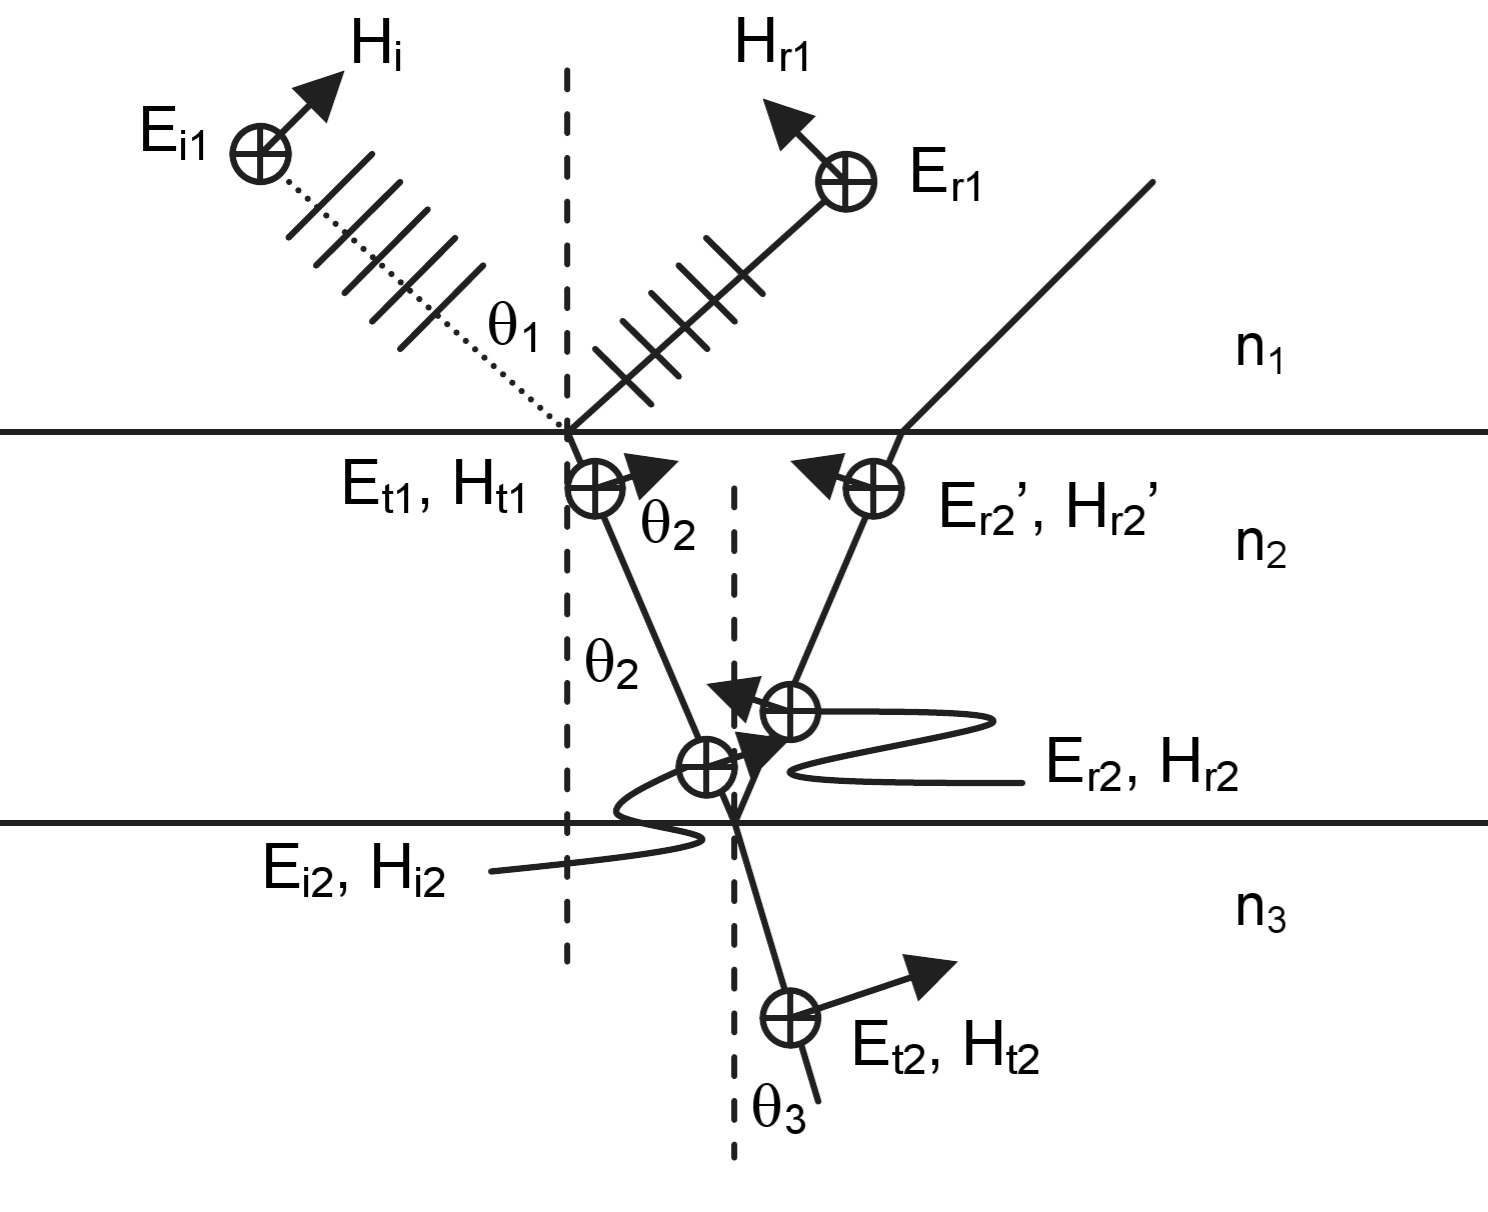
\includegraphics[height=.45\linewidth]{image2}
	\end{center}
	
	\section*{بخش اول:بررسی روابط و شرایط مرزی} 
	
	برای بررسی روابط جهت عمود بر لایه ها را $z$ در نظر گرفته و همچنین صفحه بردار $k$ را صفحه$x-z$ در نظر میگیریم.
	
	برای سادگی محاسبات قطبش $s$ را در جهت $y$ در نظر گرفته و بدین‌ترتیب قطبش $p$ در صفحه$x-z$ خواهد بود
	
	
	
	
	\section*{قطبش $s$ در مرز محیط $i$ و $i+1$:}
	
	\begin{gather*}
		n_i sin \theta_i= n _{i+1} sin \theta_{i+1}\\
		E_i+E_{ir}=E_{it}\\
		n_i cos \theta_i(	E_i-E_{ir})=n_{i+1}cos \theta_{i+1} E_{it}\\
		\Rightarrow r^s_{i,i+1}=\frac{E_{ir}}{E_i}=\frac{B_{ir}}{B_i}=\frac{n_i cos \theta_i-n_{i+1}cos \theta_{i+1}}{n_i cos \theta_i+n_{i+1}cos \theta_{i+1}}\\
		\Rightarrow t^s_{i,i+1}=\frac{E_{it}}{E_i}=\frac{n_{i+1} B_{it}}{n_i B_i}=\frac{2n_i cos \theta_i}{n_i cos \theta_i+n_{i+1}cos \theta_{i+1}}\\
		R^s=\frac{|E_{r}\cross B_{r}|}{|E\cross B|}=r^s r^{s*}\\
		T^s=\frac{|E_{t}\cross B_{t}|cos \theta_{N}}{|E\cross B|cos \theta_1}=\frac{n_Ncos \theta_N}{n_1cos \theta_1} t^s t^{s*}
	\end{gather*}
	
	که در این معادله ضرایب $r,t$  از برهمکنش موج های بازتابیده و انتقال یافته بدست می‌آیند که برای حالت بدون لایه‌نازک یا یک لایه‌نازک حل پارامتری دارد اما در غیر این صورت نیاز به حل عددی است
	
	\newpage
	\section*{قطبش $p$ در مرز محیط $i$ و $i+1$:} 
	
	\begin{gather*}
		n_i sin \theta_i= n _{i+1} sin \theta_{i+1}\\
		n_i(E_i+E_{ir})=n_{i+1}E_{it}\\
		cos \theta_i(	E_i-E_{ir})=cos \theta_{i+1} E_{it}\\
		\Rightarrow r^p_{i,i+1}=\frac{E_{ir}}{E_i}=\frac{B_{ir}}{B_i}=\frac{n_{i+1}\theta_i-n_i cos \theta_{i+1}}{n_i cos \theta_{i+1}+n_{i+1}cos \theta_i}\\
		\Rightarrow t^p_{i,i+1}=\frac{E_{it}}{E_i}=\frac{n_{i+1} B_{it}}{n_i B_i}=\frac{2n_i cos \theta_i}{n_i cos \theta_{i+1}+n_{i+1}cos \theta_i}\\
		R^p=\frac{|E_{r}\cross B_{r}|}{|E\cross B|}=r^p r^{p*}\\
		T^p=\frac{|E_{t}\cross B_{t}|cos \theta_{N}}{|E\cross B|cos \theta_1}=\frac{n_Ncos \theta_N}{n_1cos \theta_1} t^p t^{p*}
	\end{gather*}
	
	که مانند معادله قبل ، ضرایب $r,t$  از برهمکنش موج های بازتابیده و انتقال یافته بدست می‌آیند که برای حالت بدون لایه‌نازک یا یک لایه‌نازک حل پارامتری دارد اما در غیر این صورت نیاز به حل عددی است
	\\
	همچنین برای محاسبه برهمکنش ها نیاز به دانستن اختلاف فاز پس از طی کردن طول هر لایه دارد:
	\begin{gather*}
		\beta_i=d_ik_icos\theta_i=\frac{2\pi}{\lambda_i}cos\theta_i
	\end{gather*}
	
	\begin{center}
		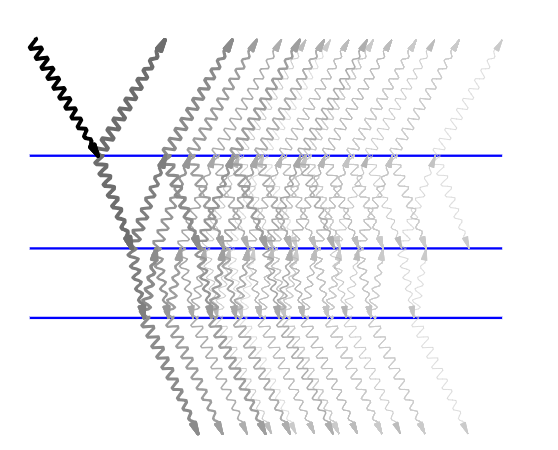
\includegraphics[height=.45\linewidth]{wAN1K}
	\end{center}
	\newpage	

	
	\section*{کاربرد تداخل امواج الکترومغناطیسی در لایه‌های‌نازک}
	\textbf{۱.پوشش های ضد بازتاب}
	\\
	
	در اینجا نیز با استفاده از تداخل ویرانگر امواج بازتاب شده، بازتاب از سطح جسم را کاهش میدهیم که از کاربرد آن میتوان به عینک های ضد انعکاس، صفحه نمایش گوشی و نمایشگر هاو افزایش جذب نور در سلول های خورشیدی اشاره نمود.
	
	حال به بررسی یک مثال برای موادی که به صورت کاربردی برا ساخت عینک های ضدانعکاس استفاده میشوند می‌پردازیم:
	
	در این مثال ضریب بازتاب با استفاده از تداخل ویرانگر در لایه ها در بازه نور مرئی صفر میشود
	
	\begin{center}
		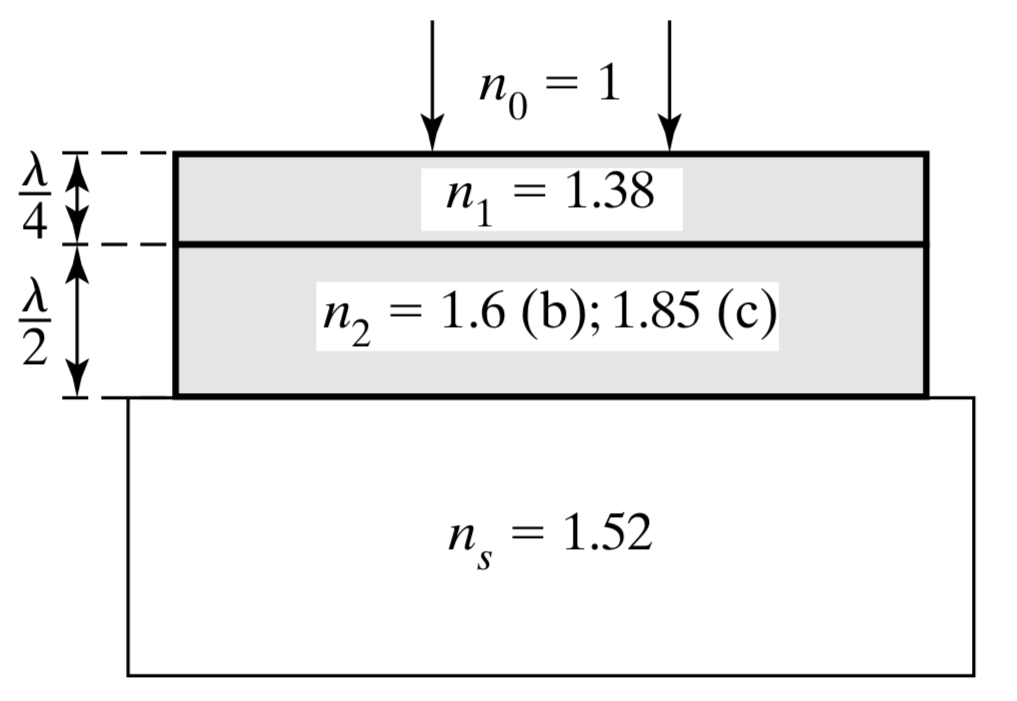
\includegraphics[height=.3\linewidth]{image_2025-07-16_20-45-14}
	\end{center}
	در کتاب اپتیک $pedrotti$ به بررسی این سسیتم در طول موج های مرئی در زاویه عمود بر سطح میپردازد که نمودار بدست آمده عبارت است از:
	\begin{center}
		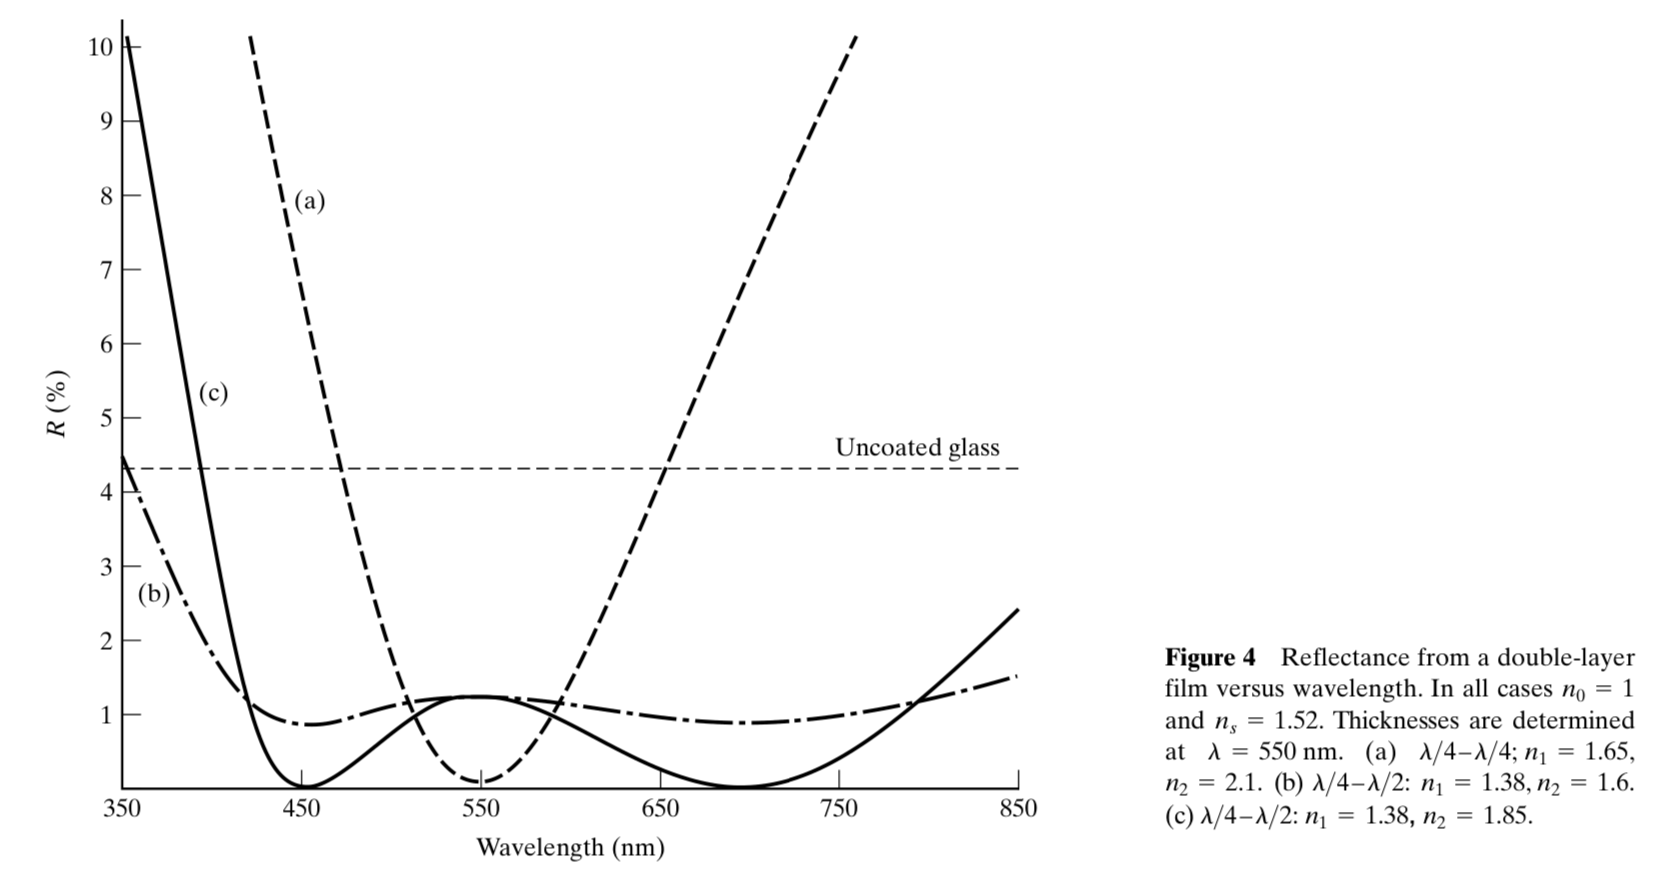
\includegraphics[height=.5\linewidth]{image_2025-07-16_20-39-13}
	\end{center}
	\newpage
	همچنین مشاهده میشود که در این مثال کد شبیه سازی نتایج یکسانی را رقم میزند
	\begin{center}
		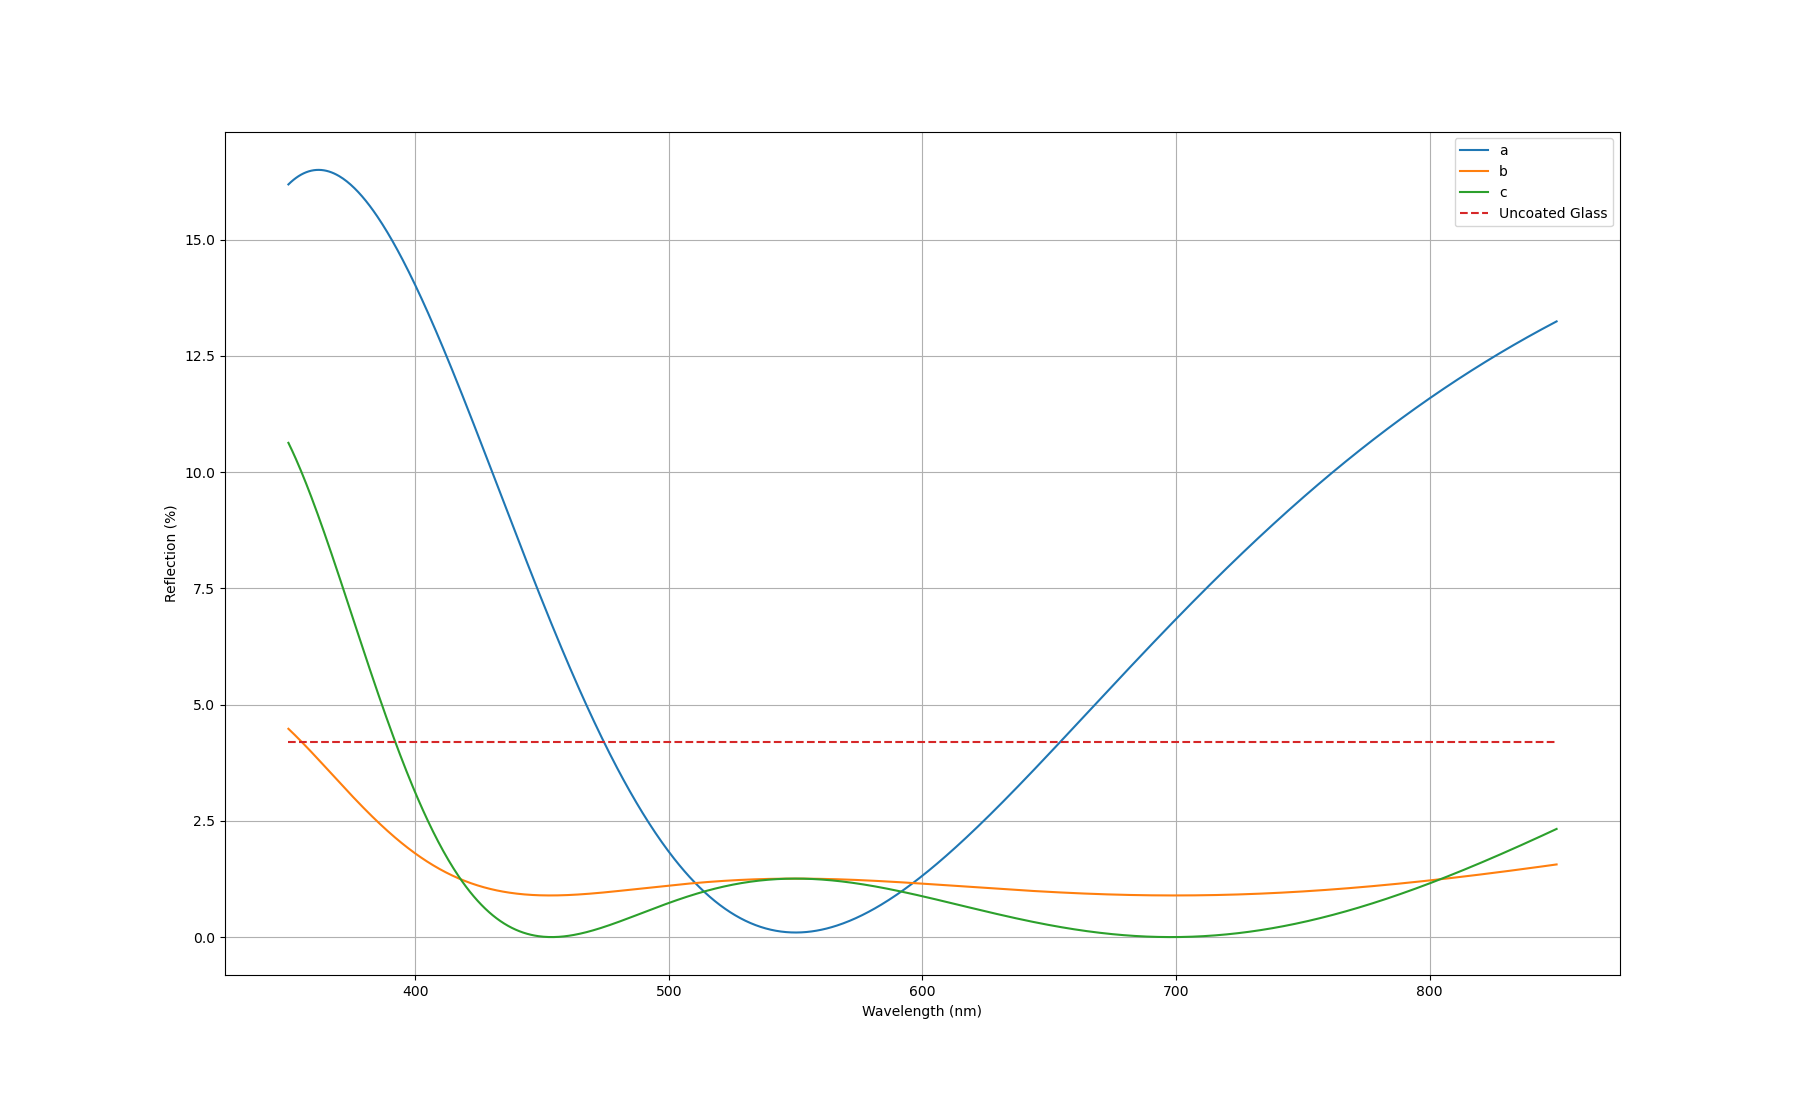
\includegraphics[height=.5\linewidth]{fig1}
	\end{center}
	
	\textbf{۲.لیزر}
	\\
	
	 در آخرین مورد از لایه‌های نازک دی‌الکتریک به عنوان پوشش داخلی کاواک لیزر استفاده میشود.
	
	این لایه ها تداخل های سازنده در فرکانس خاص ایجاد کرده که باعث تشدید فرکانس مد نظر ما میشود و به‌ گونه‌ای بازتاب در آن فرکانس به بالاترین مقدار ممکن خود خواهد رسید. 
	\newpage
	
	
	
	\section*{طرز کار الگوریتم}
		
		این الگوریتم بازتاب از سطوح نازک را با شبیه‌سازی انتشار نور به صورت برهم‌نهی امواجی که بارها در مرزها بازتاب می‌شوند و انتقال می‌یابند حساب می‌کند. این الگوریتم چند بخش مهم دارد که در ادامه توضیح داده شده‌اند.
		
	\subsection*{تقسیم موج}
		
		در هر مرز موج فرودی به دو موج بازتابی و انتقالی تقسیم می‌شود. با استفاده از معادلات فرنل شدت هر دو موج حساب می‌شود و اثربخشی موج فرودی همینجا تمام می‌شود.
		
	\subsection*{جمع شدن فازها}
		
		امواج با توجه به اختلاف مسیری که طی می‌کنند با یکدیگر دچار اختلاف فاز می‌شوند. این الگوریتم با در نظر گرفتن طول موج، ضریب شکست محیط و زاویهٔ حرکت تغییرات فاز امواج را محاسبه کرده و اثر می‌دهد.
		
	\subsection*{تداخل}
		
		در نهایت با برهم‌نهی همهٔ امواج بازتاب‌شده و در نظر گرفتن شدت و اختلاف فازشان با هم می‌توان ضریب بازتاب را محاسبه کرد.
		
	\subsection*{پایان شبیه‌سازی}
		
		هر گاه شدت یک پرتو به قدری کم بشود که قابل چشم‌پوشی باشد از شبیه‌سازی حذف می‌شود. شبیه‌سازی تا جایی ادامه می‌یابد که همهٔ پرتوها یا از لایه خارج شده باشند یا به قدری ضعیف شده باشند که قابل چشم‌پوشی باشند ($10^{-6}$ بار شدت پرتوی اولیه).
		
	\section*{راهنمای استفاده از برنامه}
		
		برای اجرای برنامه نیاز به کتابخانه‌های پایتون \lr{numpy} و \lr{matplotlib} دارید. فایل اصلی برنامه \lr{thinfilms.py} نام دارد. همچنین فایل دیگری به اسم \lr{glasses.py} نیز هست که بازتاب از یک سری لایهٔ از پیش تعریف شده را محاسبه کرده و روی نمودار نشان می‌دهد.
		
		پس از اجرا کردن فایل اصلی یک سری سؤال از شما پرسیده می‌شود که باید مانند شکل زیر پاسخ بدهید:
		
	\begin{center}
		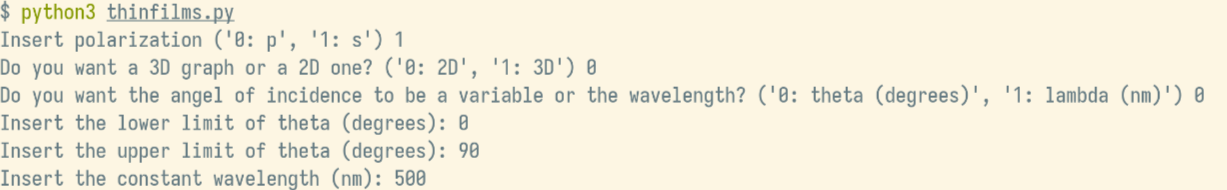
\includegraphics[height=0.15\linewidth]{questions.png}
	\end{center}
		
		پس از دادن جواب همهٔ سوال‌ها منتظر بمانید تا محاسبات تمام شوند و نمودار نشان داده شود.
		
		برای تغییر دادن لایه‌های استفاده شده در شبیه‌سازی می‌توانید متغیر \lr{films} را مشابه نمونهٔ زیر تغییر بدهید:
		
	\begin{latin}
		\begin{minted}{python}
            films = [[1,     0],     # First layer n_0
                    [2.25,  300],
                     ...
                    [k (Dielectric Constant), d (Film Thickness)],
                    ...
                    [2.3104, 0]]   # Last layer  n_s
		\end{minted}
	\end{latin}
	
	
	
	
	
	
	
	
	
\end{document}

